%-------------------------------------------------------------------------------
%-------------------------------------------------------------------------------
\begin{frame}
	\textbf{Generalized Roy model}
	\begin{align*}\begin{array}{l@{\qquad}l}
			\text{Potential Outcomes} &\text{Observed Outcome}\\
			Y_1 = \mu_1(X) + U_1      &  Y = D Y_1 + (1 - D)Y_0 \\
			Y_0 = \mu_0(X) + U_0      &\\
			& \\
			\text{Choice} & \\
			D = \mathrm{I}[\mu_D(X, Z) - V > 0] & \\
		\end{array}
	\end{align*}
\end{frame}
%-------------------------------------------------------------------------------
%-------------------------------------------------------------------------------
\begin{frame}
	\begin{figure}[htp]\centering
		\caption{Treatment Effects}\scalebox{0.35}{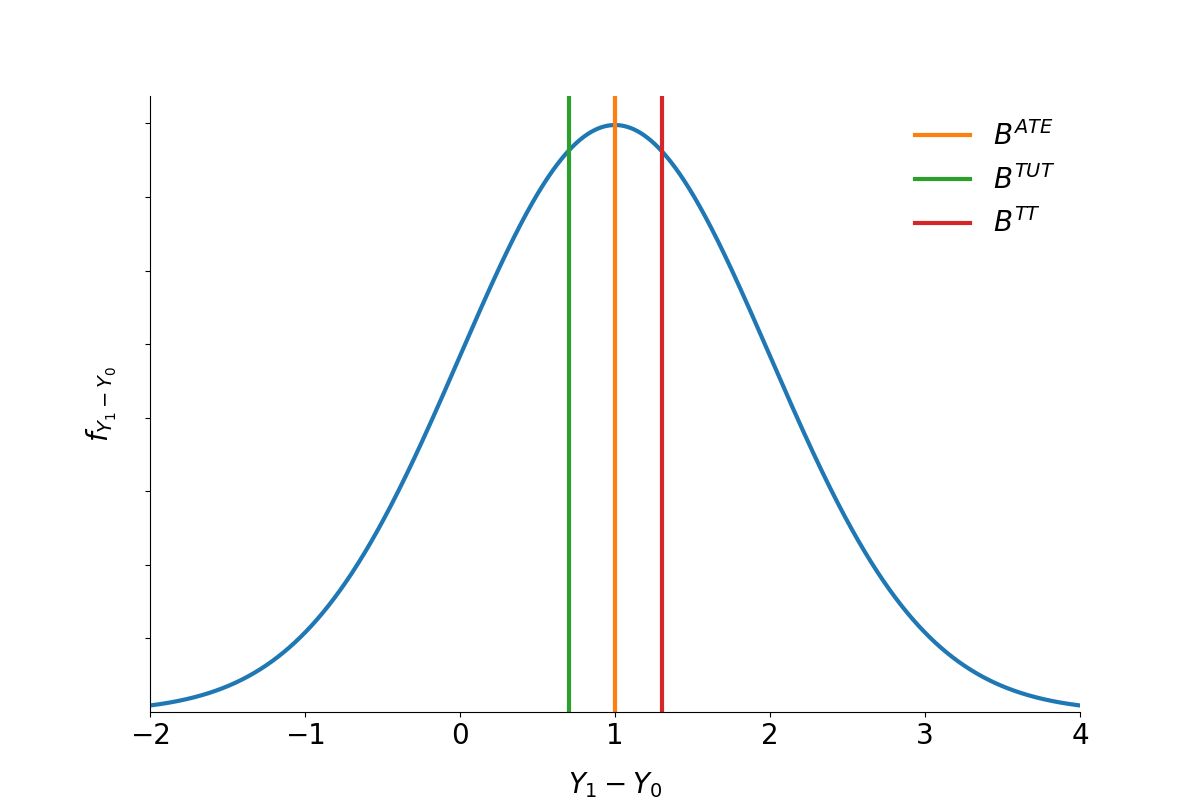
\includegraphics{fig-treatment-effects-with-eh}}
	\end{figure}
\end{frame}
%-------------------------------------------------------------------------------
%-------------------------------------------------------------------------------
\begin{frame}
	\frametitle{Teaching Tool}
	\begin{figure}[htp]\centering
		
\includegraphics[width=\textwidth]{fig-online-documentation-grmpy}
	\end{figure}
\end{frame}
